\chapter{Desarrollo de Aplicaciones}
\label{desarrollo}

En este capítulo se hablará sobre las diferentes librerías que se han realizado en este proyecto, explicando detalladamente la estructura de cada una de ellas.

Primeramente se explicará J-OSMClient, que es el cliente programado en Java para comunicarse con la \ac{REST}-\ac{API} que exporta \ac{OSM}.

Seguidamente se hablará de J-ONOSClient, que es el cliente encargado de comunicarse con la \ac{REST}-\ac{API} de \ac{ONOS}, y de J-OpenStack Client, que se encarga de comunicarse con la \ac{REST}-\ac{API} de OpenStack.

Por último, se hará especial énfasis en el plugin de Net2Plan desarrollado, en el cual se han integrado las diferentes \acp{API} mencionadas anteriormente.


\section{J-OSM Client}
\label{sec:osmclient}

J-OSMClient\cite{josmclientbib} es una librería programada en Java cuya funcionalidad es la de proporcionar un cliente \ac{REST} para interactuar con \ac{OSM} (ver \ref{sec:osm}). Está basado en el cliente programado en Python por la \ac{ETSI} (ver \ref{subsec:osmclientpython}).

Se compone principalmente de tres clases que realizan la comunicación con \ac{OSM} y devuelven los resultados de las interacciones al usuario:

\begin{itemize}
	\item \textbf{OSMControllerRelease3:} Es la entidad que se encarga de realizar la comunicación con la \textit{release} 3 de \ac{OSM}. Mediante llamadas \ac{HTTP} (GET, POST, PUT, DELETE), dicha clase envía peticiones y procesa internamente las respuestas recibidas.
	
	\item \textbf{OSMControllerSOL005:} Esta entidad se encarga de realizar la comunicación con la \textit{release} 4 en adelante, utilizando el estándar sol005\cite{sol005item}. Al igual que el \textit{controller} de la \textit{release} 3, establece la comunicación con llamadas \ac{HTTP} enviando peticiones y procesando las diferentes respuestas recibidas.
	
	\item \textbf{OSMClient:} Es la clase principal de la aplicación. Actúa como interfaz entre el usuario final y los \textit{controllers}, permitiendo que el usuario obtenga directamente en formato más amigable las respuestas dadas por el servidor de \ac{OSM}.
\end{itemize}

\clearpage

\begin{figure}[!ht]
	\centering
	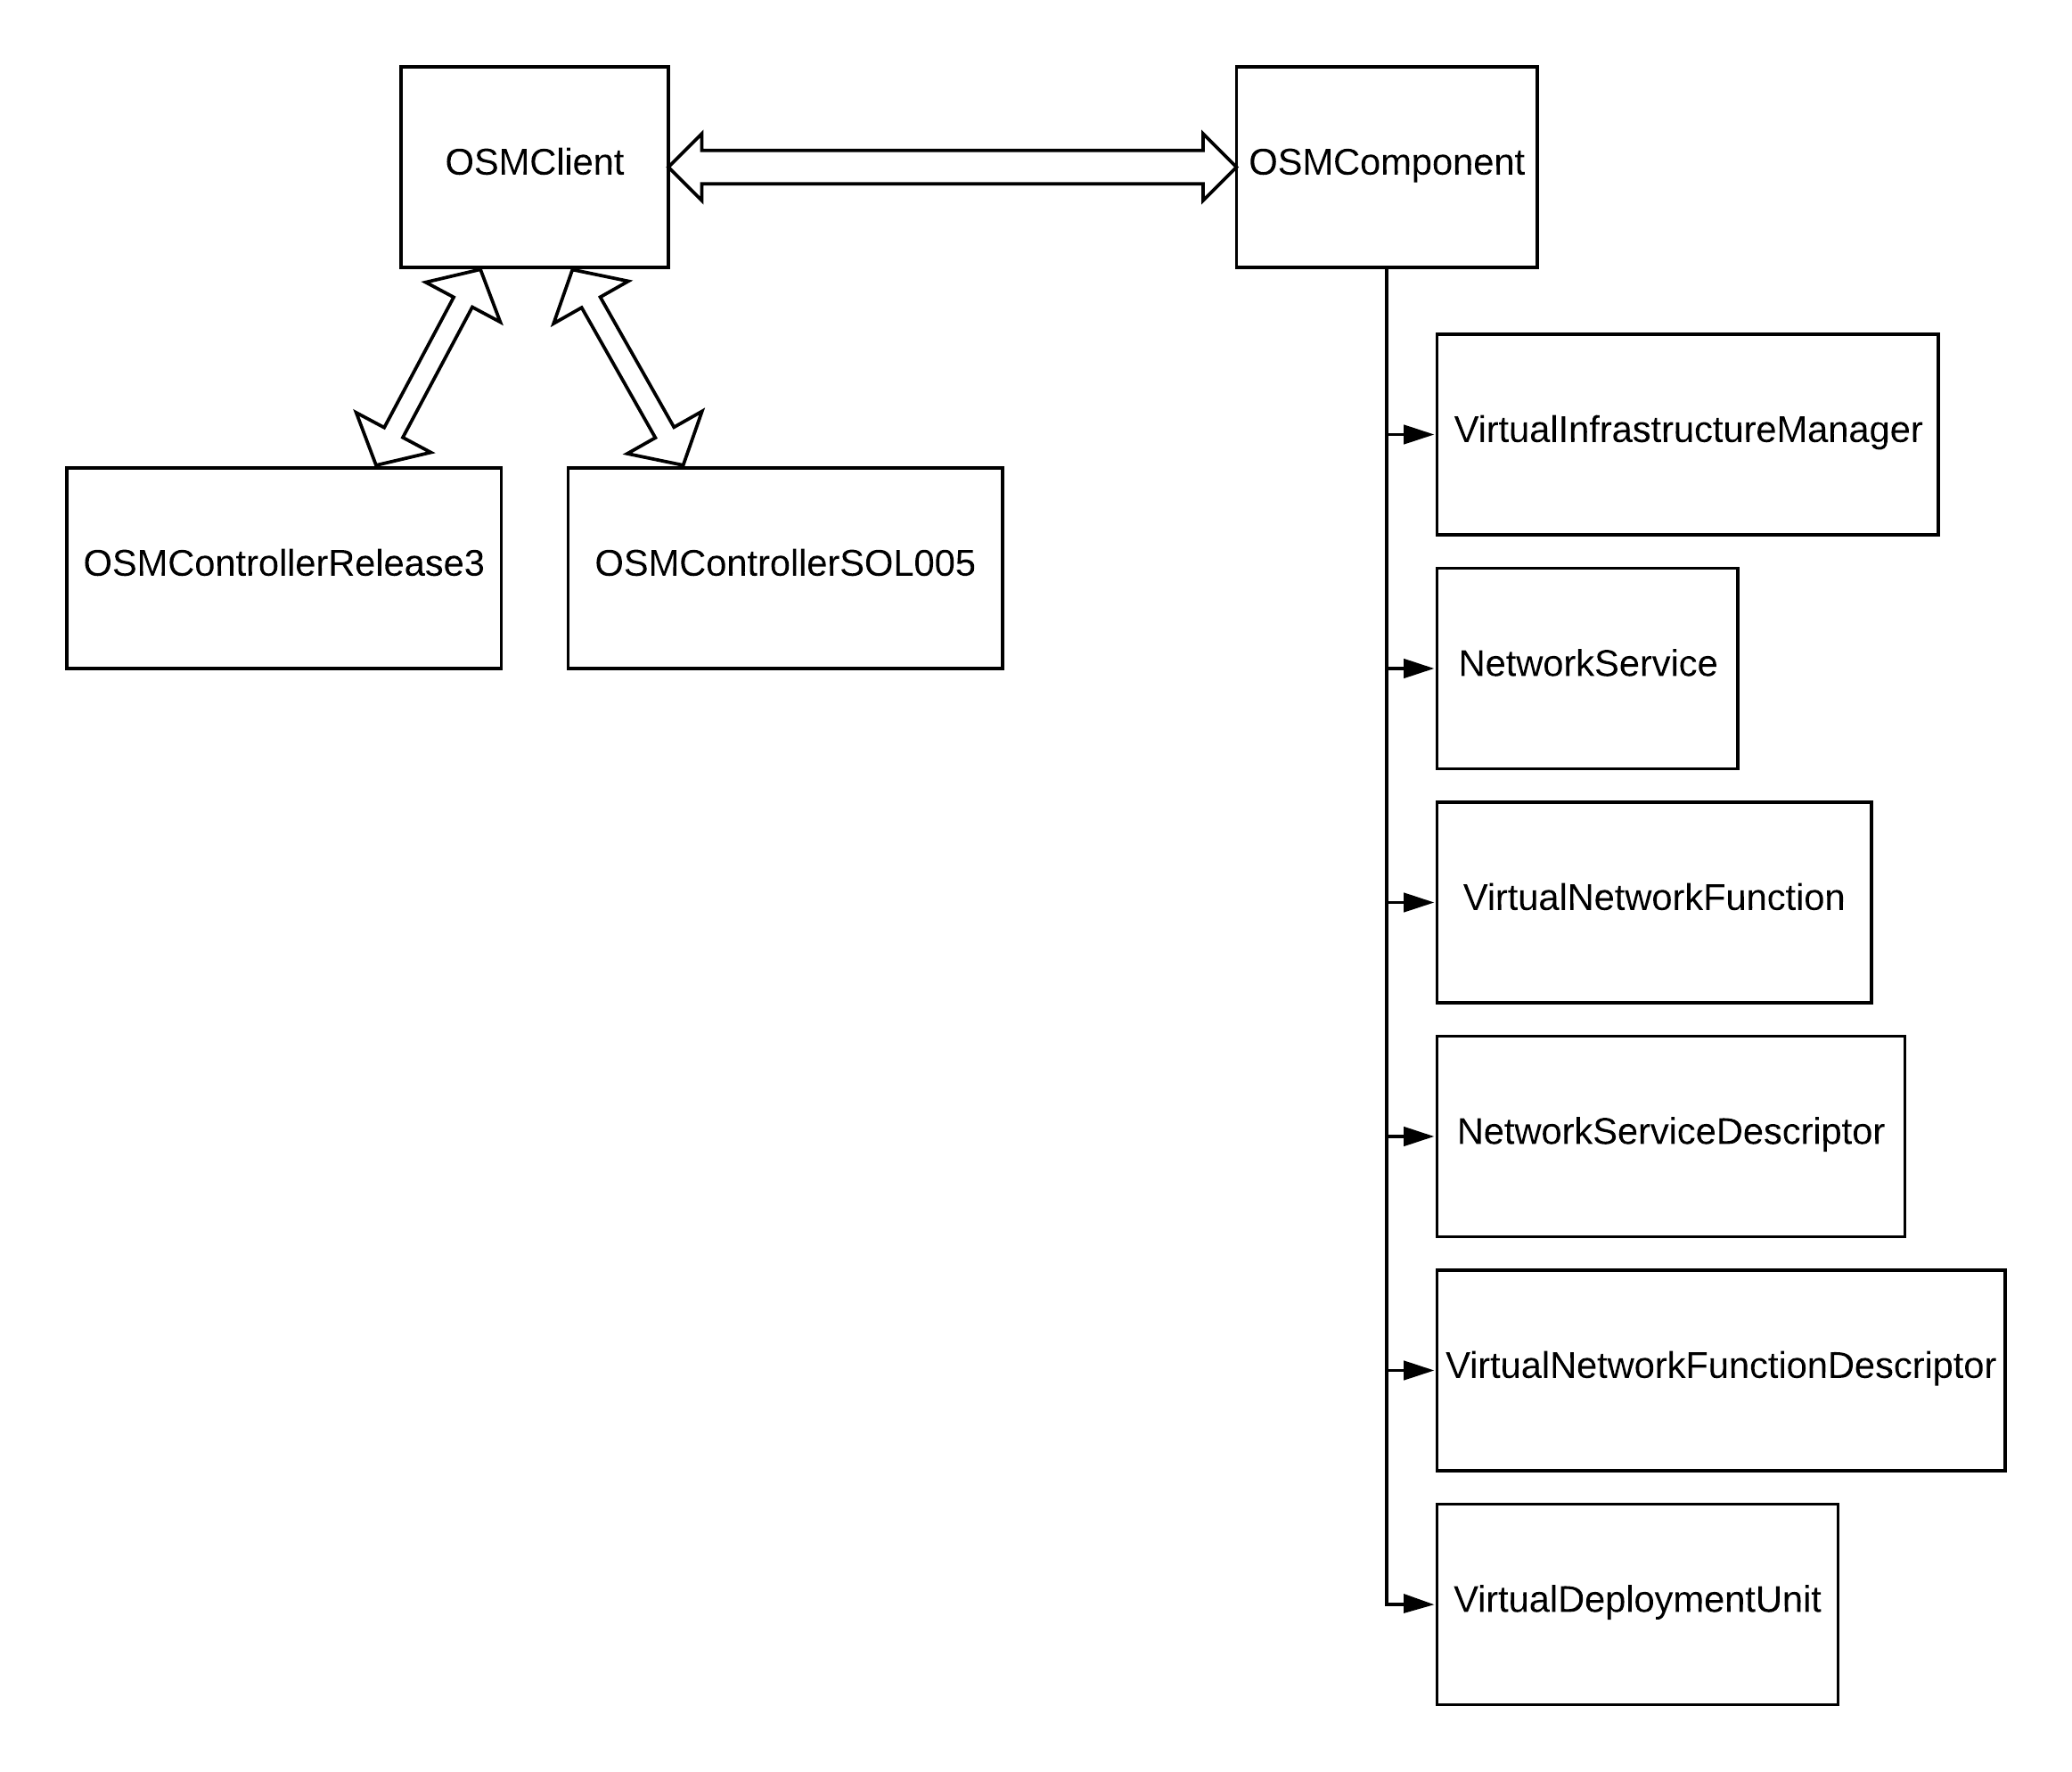
\includegraphics[width=1\linewidth]{imagenes/OSMClient}
	\caption{Estructura de clases de J-OSMClient}
	\label{fig:osmclient}
\end{figure}

En la figura \ref{fig:osmclient} se puede ver un esquema detallado de la jerarquía de clases. Se aprecia como OSMClient interactúa directamente con ambos \textit{controllers} para establecer la comunicación con ambas versiones de \ac{OSM}.

Así mismo, se pueden observar las clases auxiliares que definen los diferentes componentes internos de \ac{OSM}. Estas clases existen debido a que \ac{OSM} envía las respuestas \ac{HTTP} con un formato \ac{JSON}, que no es el formato óptimo para que el usuario final las reciba y las trate.

Estas clases auxiliares se explican a continuación:

\begin{itemize}
	\item \textbf{OSMComponent:} Es la clase genérica que define un componente de \ac{OSM}. Todas las demás clases heredan de ella, lo que permite un mejor procesamiento interno de las respuestas recibidas de \ac{OSM}, ya que proveé atributos comunes a todos los componentes, como nombre o identificador interno.
	
	\item \textbf{VirtualInfraestructureManager:} Esta clase es la que modela el componente \ac{VIM}. Proveé atributos como su \ac{URL} y su tipo (OpenStack, OpenVim, VMWare o \ac{AWS}).
	
	\item \textbf{VirtualLinkDescriptor:} Esta clase es la que define el componente \ac{VLD}. Proporciona un único atributo, que es una lista de conexiones en las que se indica los dos puertos que se conectan gracias a él.
	
	\item \textbf{VirtualDeploymentUnit:} Esta clase define el componente \ac{VDU}. Proveé diferentes atributos como la imagen que lo define y los recursos necesarios para su creación (\ac{HD}, \ac{CPU} y \ac{RAM}).
	
	\item \textbf{VirtualNetworkFunctionDescriptor:} Esta clase es la que modela el componente \ac{VNFD}. Proporciona únicamente un atributo, que es la lista de \acp{VDU} que lo componen.
		
	\item \textbf{VirtualNetworkFunction:} Esta clase define el componente \ac{VNF}. Proveé diferentes atributos, como el \ac{NS} al que pertenece, el \ac{VIM} donde está instanciado o el \ac{VNFD} que lo define, entre otros.
	
	\item \textbf{NetworkServiceDescriptor:} Esta clase es la que modela el componente \ac{NSD}. Proporciona diferentes atributos, como la lista de \acp{VNFD} que lo componen o la lista de \acp{VLD}.
	
	\item \textbf{NetworkService:} Esta clase modela el componente \ac{NS}. Está compuesto de diferentes atributos, como los \acp{VIM} donde está instanciados sus \acp{VNF}, el \ac{NSD} que lo define, la lista de \acp{VNF} que lo forman o su estado actual.
	
\end{itemize}


\section{J-ONOS Client}
\label{sec:onosclient}

J-ONOSClient\cite{onosjavadocbib} es una librería programada en Java cuya funcionalidad es la de proporcionar un cliente \ac{REST} para interactuar con \ac{ONOS} (ver \ref{sec:onos}). Esta librería está basada en la representación de objetos que proveé Swagger (ver \ref{subsec:openapi}). Gracias a Swagger, se ha generado un cliente que es capaz de interactuar con \ac{ONOS}.

Este cliente generado proveé una representación de diferentes componentes, cada uno de ellos con una clase asociada que actúa como interfaz con \ac{ONOS} para controlar las interacciones que involucran a dicho componente. A continuación se explica cada uno de los componentes mencionados anteriormente:

\begin{itemize}
	
	\item \textbf{Host:} Este componente representa un usuario final en una red, más concretamente una \ac{NIC}. Proporciona diferentes atributos como su identificador interno, su dirección \ac{IP}, su dirección \ac{MAC} o el identificador de la \ac{VLAN} a la que pertenece.
	
	\item \textbf{Device:} Este componente es una representación de un dispositivo perteneciente a la infraestructura de red. Proporciona los siguientes atributos: su identificador interno, un identificador de \textit{chassis}, un número de serie único, el identificador del fabricante, un número de versión de \textit{hardware}, un número de versión de \textit{software} y el tipo de dispositivo. 
	
	\item \textbf{Port:} Este componente representa un puerto físico de red. Proveé al usuario de distintos atributos, entre los que destacan el dispositivo al que pertenece, el número de puerto, la velocidad que soporta y el tipo de puerto.
	
	\item \textbf{Link:} Este componente es una representación de un enlace entre dos dispositivos de la infraestructura de red. Proporciona los siguiente atributos: el dispositivo origen y el dispositivo destino, el estado del enlace y el tipo de enlace.
	
	\item \textbf{Flow:} Este componente representa una regla de flujo que se aplica en un dispositivo concreto. Proveé al usuario de distintos atributos, como su identificador interno, el selector y el tratamiento que lo componen y si es permanente o no, entre otros.
	
	\item \textbf{Intent:} Este componente es una representación de una combinación origen-destino. Gracias a él, el usuario puede definir un nodo origen y un nodo destino entre los cuales se cursará una demanda de tráfico, y \ac{ONOS} traduce dicho \textit{intent} a un conjunto de reglas de flujo totalmente transparentes al usuario, sin necesidad de crearlas automáticamente. Proporciona diversos atributos, entre los que destacan su identifcador interno, su prioridad y si ha sido posible llevarlo a cabo (si no existe un camino entre el origen y el destino, la instalación del \textit{intent} fallará).
	
\end{itemize}


\begin{figure}[!ht]
	\centering
	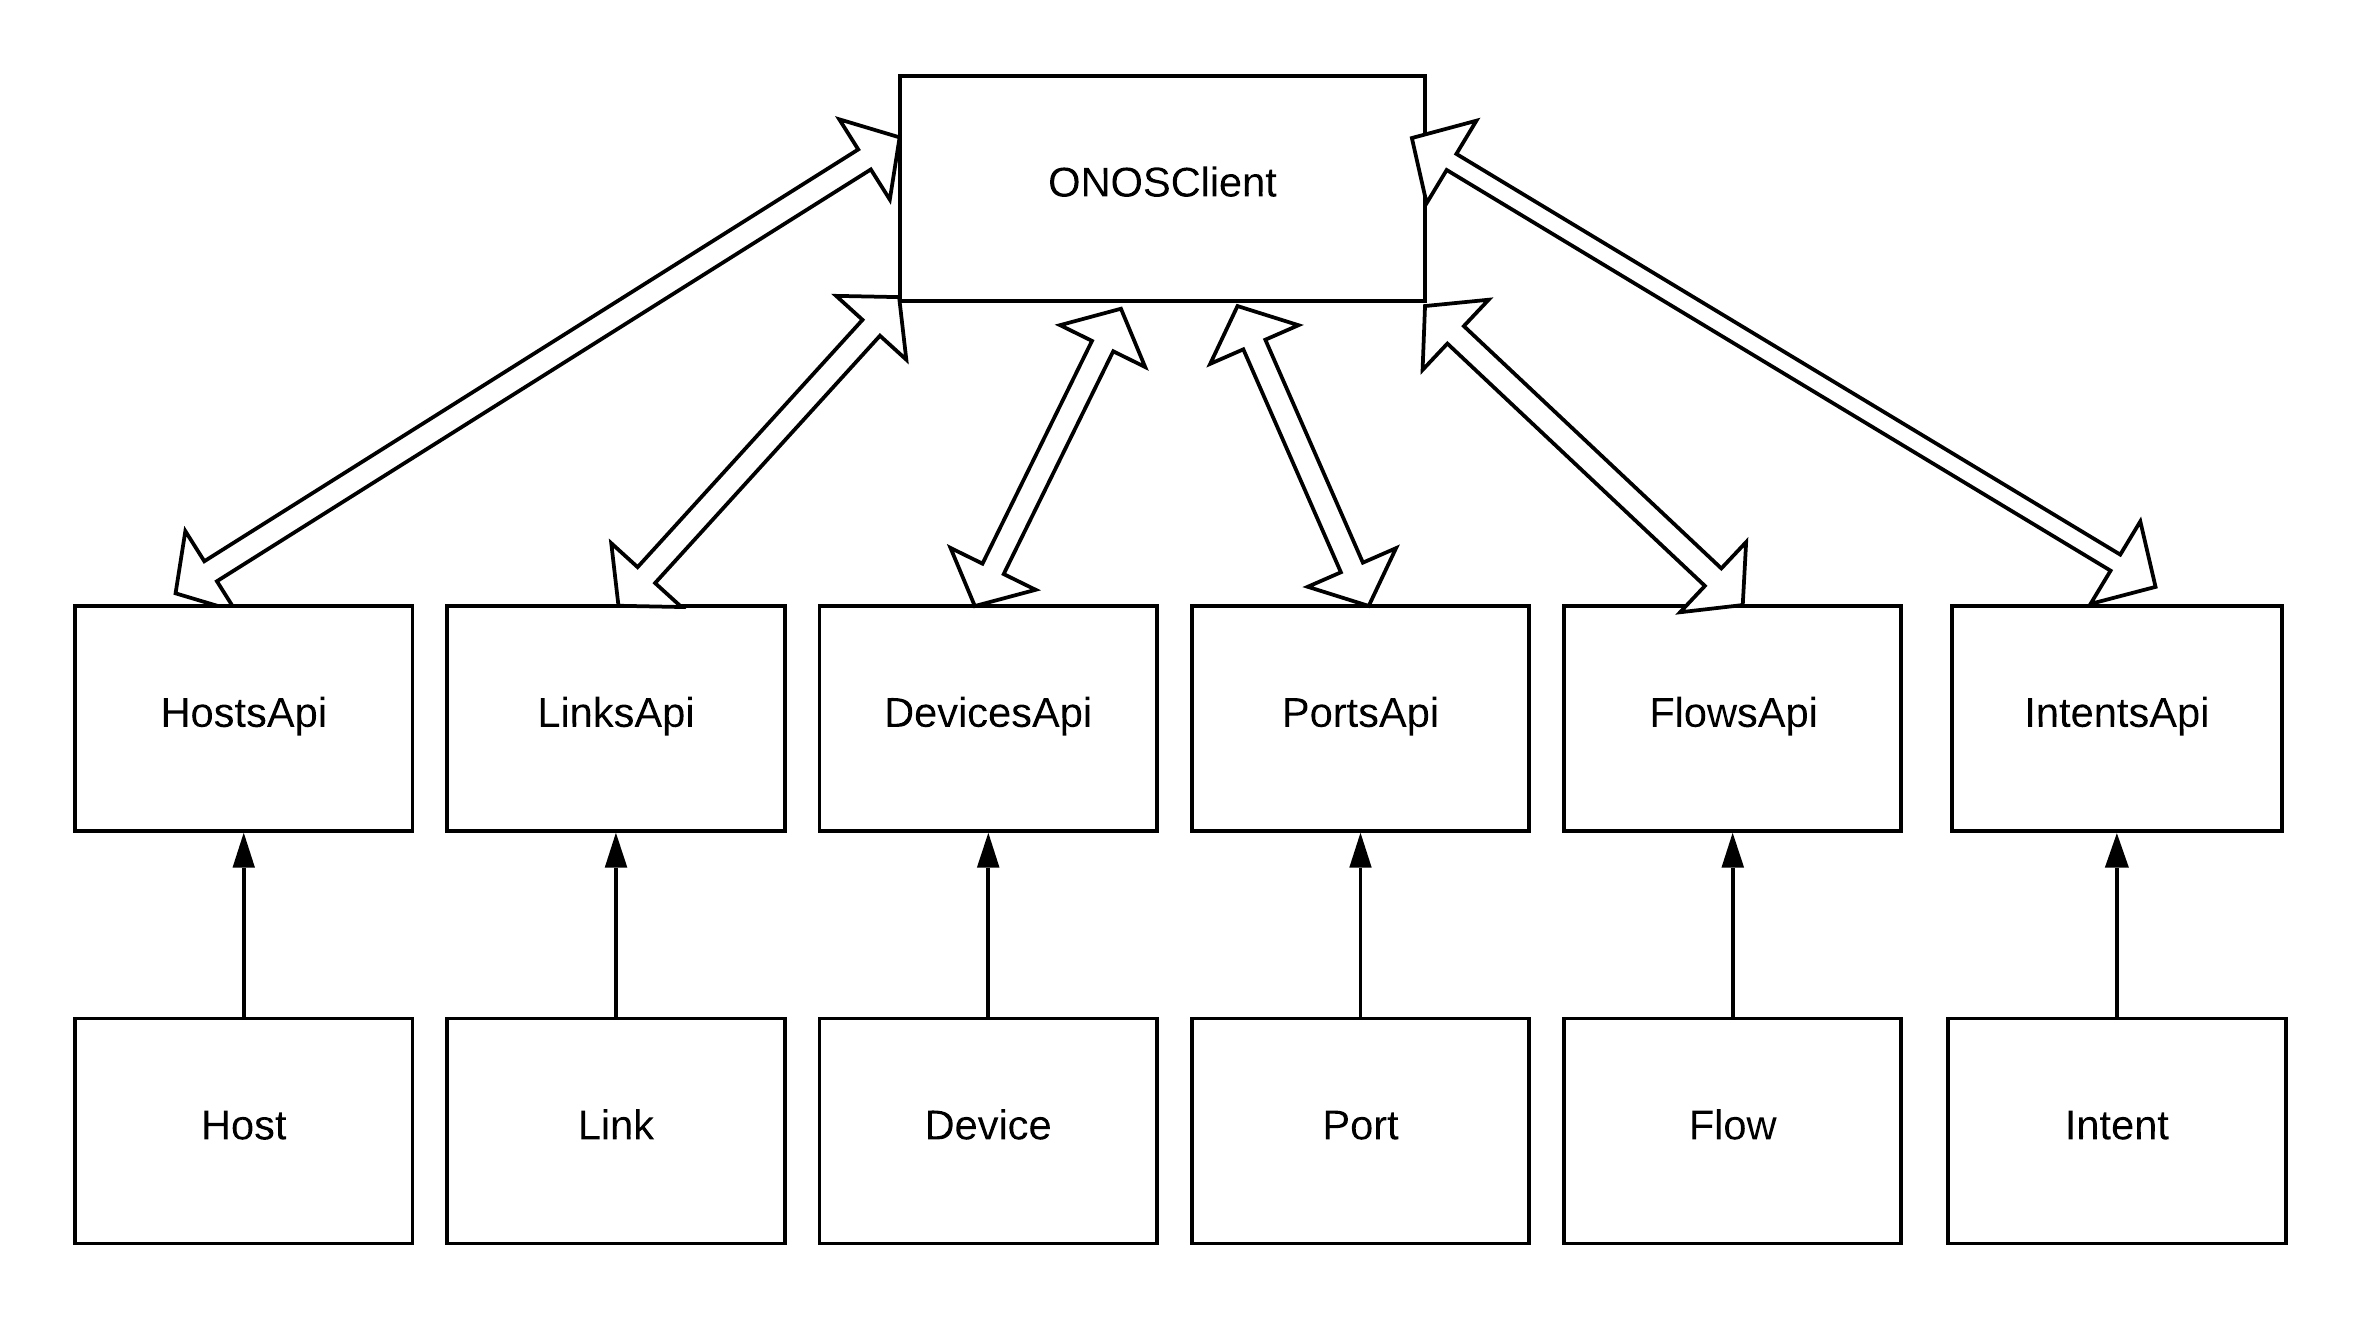
\includegraphics[width=1\linewidth]{imagenes/ONOSClient}
	\caption{Estructura de clases de J-ONOSClient}
	\label{fig:onosclient}
\end{figure}

En la figura \ref{fig:onosclient} se puede apreciar un esquema de la jerarquía de clases. Se puede observar como cada componente tiene su propia \ac{API} y todas ellas son utilizadas por la clase ONOSClient.

ONOSClient es la clase principal del cliente que actúa como interfaz entre el usuario y \ac{ONOS} interactuando con la \ac{REST}-\ac{API} de \ac{ONOS} mediante las \acp{API} de los diferentes componentes.

Dicha clase es necesaria, ya que Swagger genera varias \acp{API}, cada una de ellas para controlar las interacciones que involucran a un componente específico, pero no permite relacionar los componentes entre sí, de manera que, por ejemplo, para replicar una topología completa con todos los componentes, sin la clase ONOSClient sería imposible agruparlos.

Como ejemplo, si el cliente quiere obtener información sobre un \textit{device} en concreto, ONOSClient realizará una llamada a la clase DevicesApi, que internamente realizara una petición \ac{HTTP} GET a una \ac{URL} determinada para obtener la información buscada. La propia \ac{API} realizará una conversión de \ac{JSON} al objeto \textit{device} para proporcionar un mejor manejo de datos al usuario.


\section{J-OpenStack Client}
\label{sec:openstackclient}

J-OpenStackClient\cite{openstack4jjavadocbib} es una librería programada en Java cuya funcionalidad es la de proporcionar un cliente \ac{REST} para interactuar con OpenStack (ver \ref{sec:openstack}). Esta librería es un \textit{wrapper} de la librería \textit{open-source} OpenStack4Java (ver \ref{subsec:openstack4j}).


\begin{figure}[!ht]
	\centering
	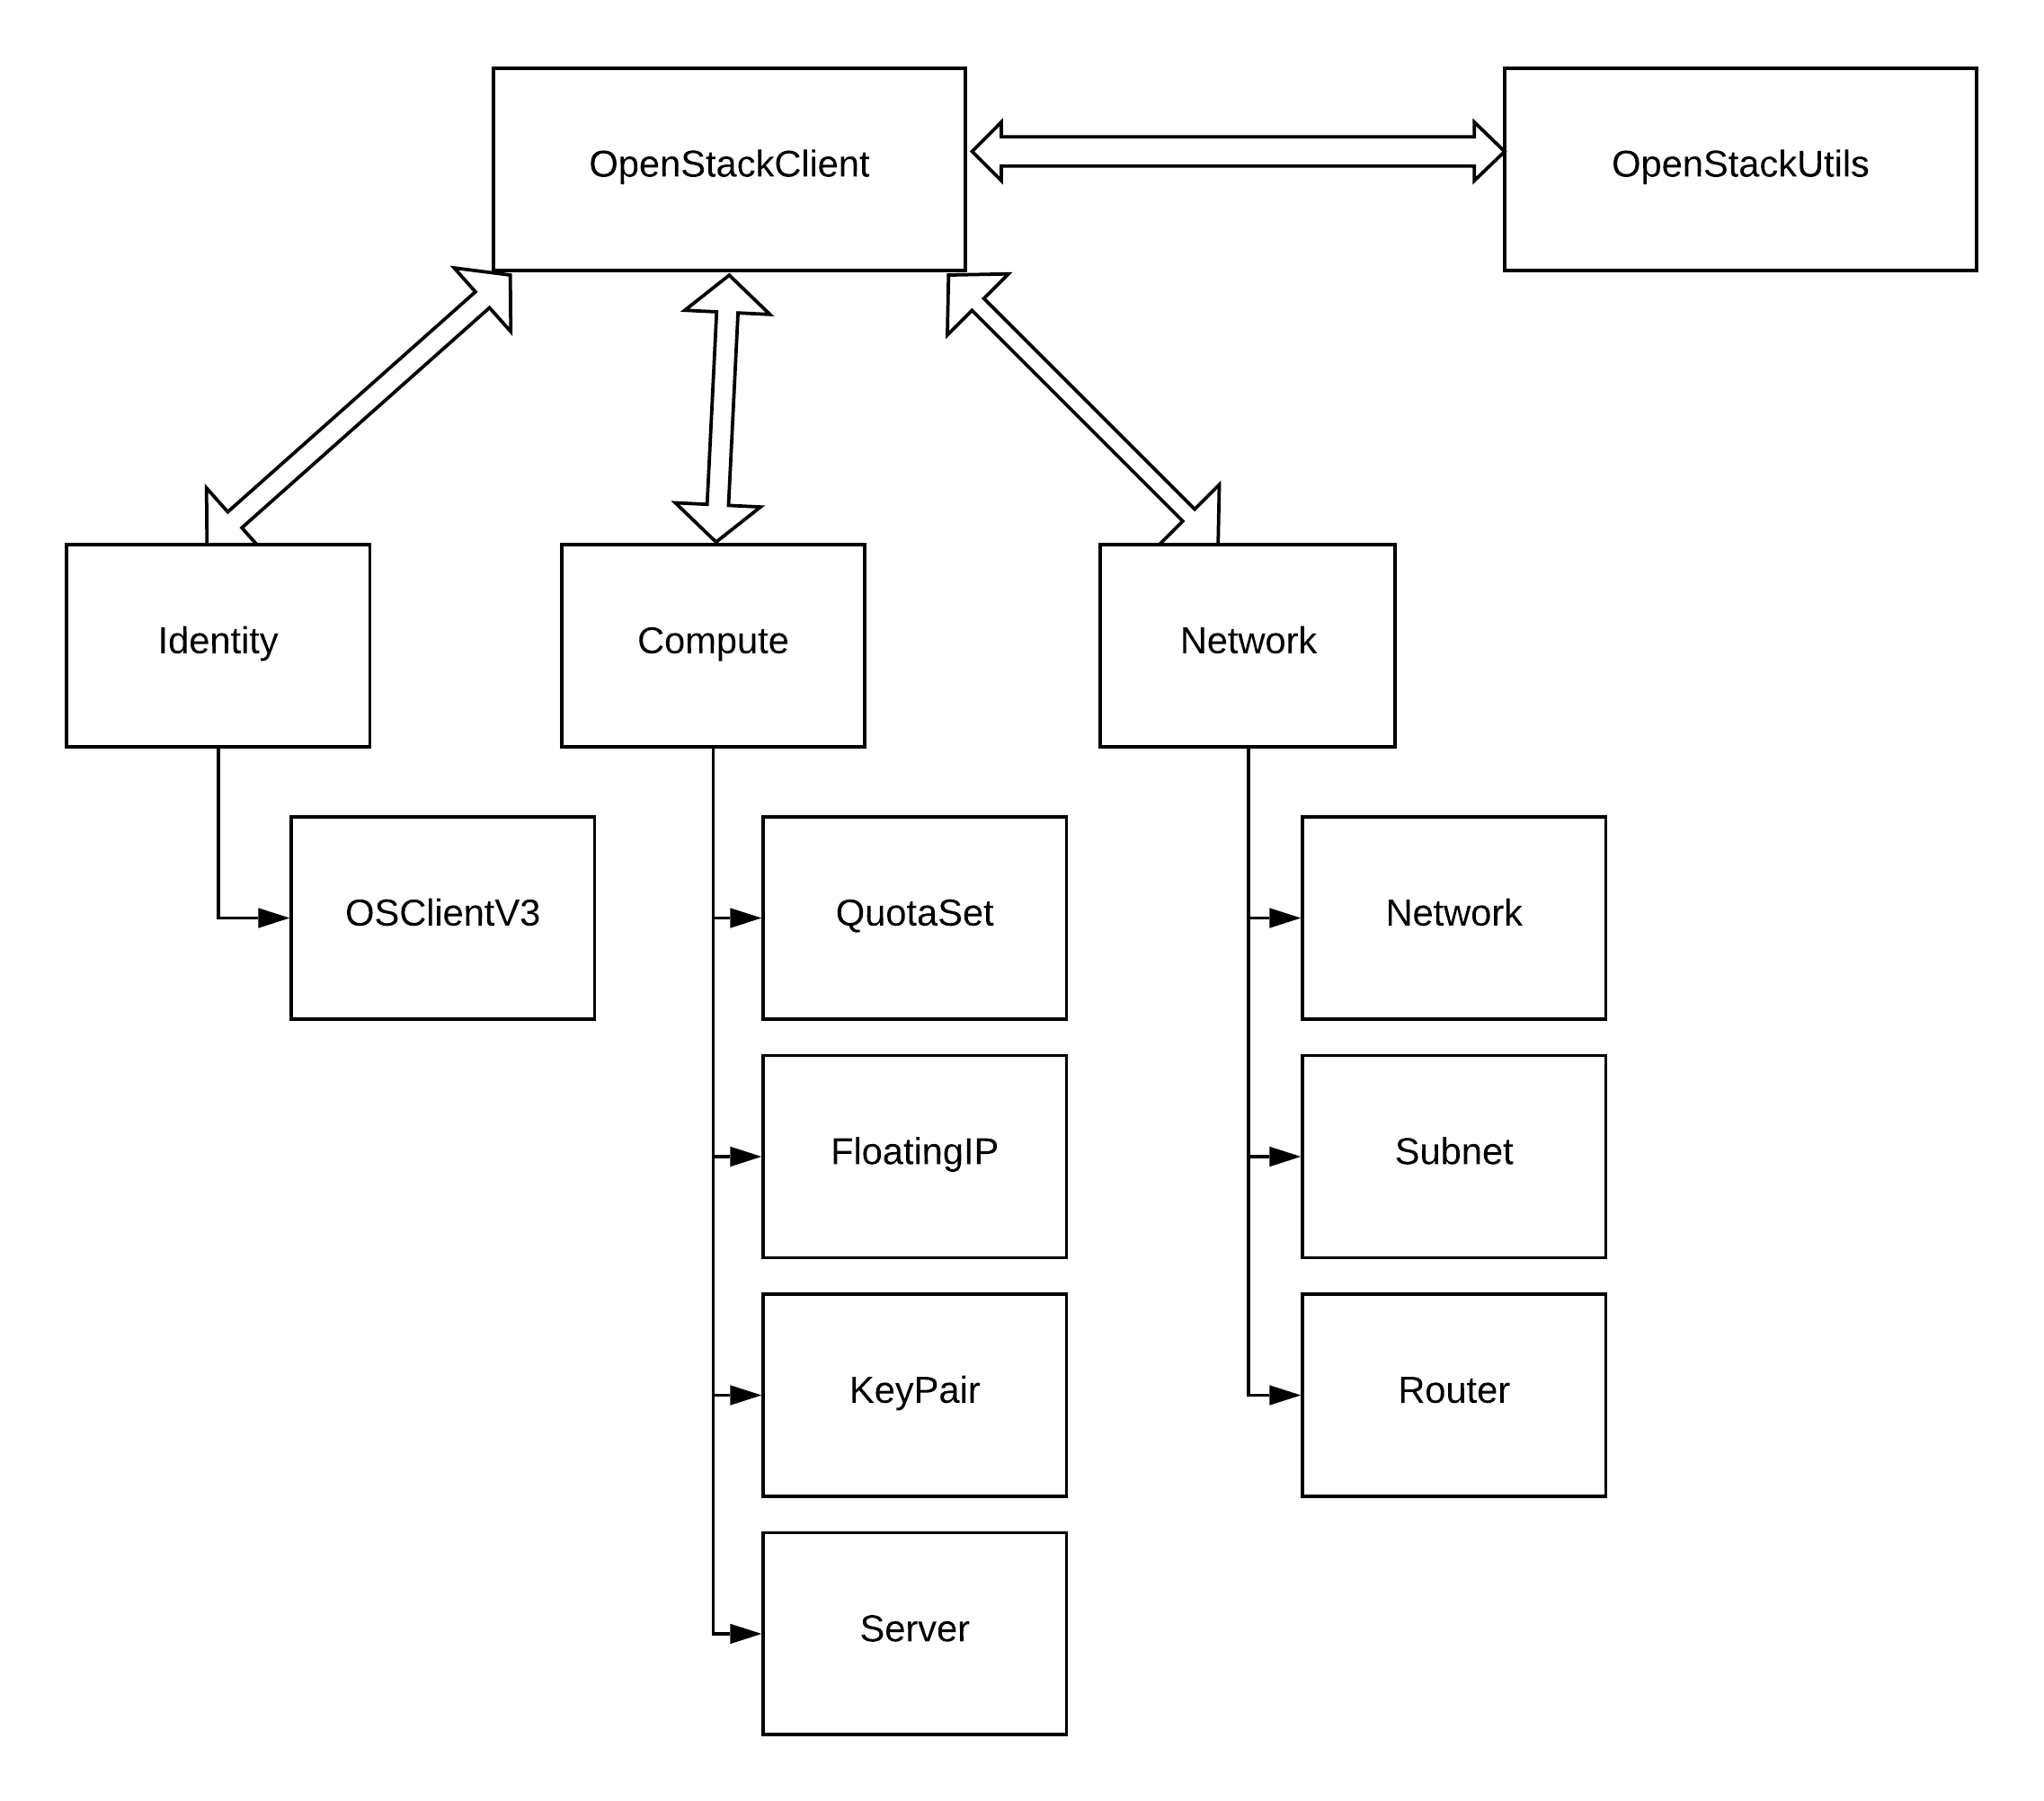
\includegraphics[width=1\linewidth]{imagenes/OpenStackClient}
	\caption{Estructura de clases de J-OpenStackClient}
	\label{fig:openstackclient}
\end{figure}

Cada uno de los servicios de OpenStack tiene una representación en este cliente, como se puede apreciar en la jerarquía de clases mostrada en la figura \ref{fig:openstackclient}. A su vez, cada servicio gobierna una serie de clases que modelan los diferentes componentes internos de OpenStack. 

Toda estas funcionalidades de los diferentes servicios son adquiridas de OpenStack4Java. El principal trabajo en este cliente es el de generar una clase central que, utilizando las clases asociadas a los diferentes servicios, permita al usuario controlar las interacciones entre ellos y sus componentes de una manera amigable y sencilla.

A continuación se realiza una explicación de la jerarquía de clases perteneciente a J-OpenStackClient:

\begin{itemize}
	
	\item \textbf{OpenStackClient:} Es la clase principal de J-OpenStackClient. Actúa como interfaz entre el usuario y las diferentes \acp{API} que controlan a su vez las interacciones con los diferentes componentes.
	
	\item \textbf{Identity:} Esta clase abstracta es la que modela el servicio KeyStone de OpenStack. Proporciona acceso al resto de servicios de OpenStack mediante autenticación por usuario-contraseña, gracias a laS clases OSClienteV2, la cual se encuentra deprecada y no se usa en las versiones actuales de OpenStack, y OSClientV3.
	
	\begin{figure}[!ht]
		\centering
		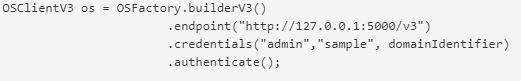
\includegraphics[width=0.8\linewidth]{imagenes/authOSClientV3}
		\caption{Autenticación mediante OSClientV3. Fuente:\cite{openstack4jbib}}
		\label{fig:authosclientv3}
	\end{figure}
	
	En la figura \ref{fig:authosclientv3} se puede apreciar un ejemplo de autenticación mediante la clase mencionada anteriormente. 
	
	\item \textbf{Compute:} Esta clase abstracta es la que modela el servicio Nova de OpenStack. Proporciona funcionalidad de gestión sobre las diferentes máquinas virtuales y su configuración. Para ello, se apoya en diferentes clases, entre las que destacan:
	
	\begin{itemize}
		
		\item \textbf{Server:} Esta clase modela una máquina virtual que está corriendo en OpenStack. 
		
		\item \textbf{FloatingIP:} Esta clase modela una dirección \ac{IP} flotante, que se utiliza para que una máquina virtual sea accesible desde el exterior (su uso es similar a \ac{NAT}).
		
		\item \textbf{KeyPair:} Esta clase modela un par de claves pública-privada para acceder a una máquina virtual mediante \ac{SSH}.
		
		\item \textbf{QuotaSet:} Esta clase modela los recursos perteneciente a una máquina virtual, tales como número de CPU, memoria RAM, almacenamiento HD, \ac{IP}s flotantes, entre otros.
		
		
	\end{itemize}
		
	\item \textbf{Network:} Esta clase abstracta modela el servicio Neutron de OpenStack. Proporciona un control sobre los componentes perteneciente a la infraestructura de red. Para ello, se apoya en las siguientes clases:
	
		\begin{itemize}
		
		\item \textbf{Network:} Esta clase modela una red, que está compuesta por diferentes subredes y por \textit{routers} para encaminar el tráfico entre diferentes subredes.
		
		\item \textbf{Subnet:} Esta clase modela una subred, que es una subdivisión de una red. Una subred tiene su propia dirección \ac{IP} y su máscara de red.
		
		\item \textbf{Router:} Esta clase es la que modela un \textit{router}, que se encarga de encaminar el tráfico entre diferentes subredes.
		
		\end{itemize}
	
	\item \textbf{OpenStackUtils:} Es una clase auxiliar que complementa a OpenStackClient. Proporciona métodos amigables para obtener atributos de los diferentes componentes de OpenStack que de forma normal sería tedioso el obtenerlos.
	
	
\end{itemize}

\section{Net2Plan: NFV Management Plugin}
\label{sec:nfvplugin}

Para llevar a cabo este proyecto, era necesario integrar las APIs mencionadas anteriormente con una herramienta que tenga funcionalidad de planificación de redes. Por ello, se ha desarrollado una extensión de Net2Plan basada en el plugin Network Design para llevar a cabo la prueba de concepto (ver \ref{pruebaconcepto}). 


\begin{figure}[!ht]
	\centering
	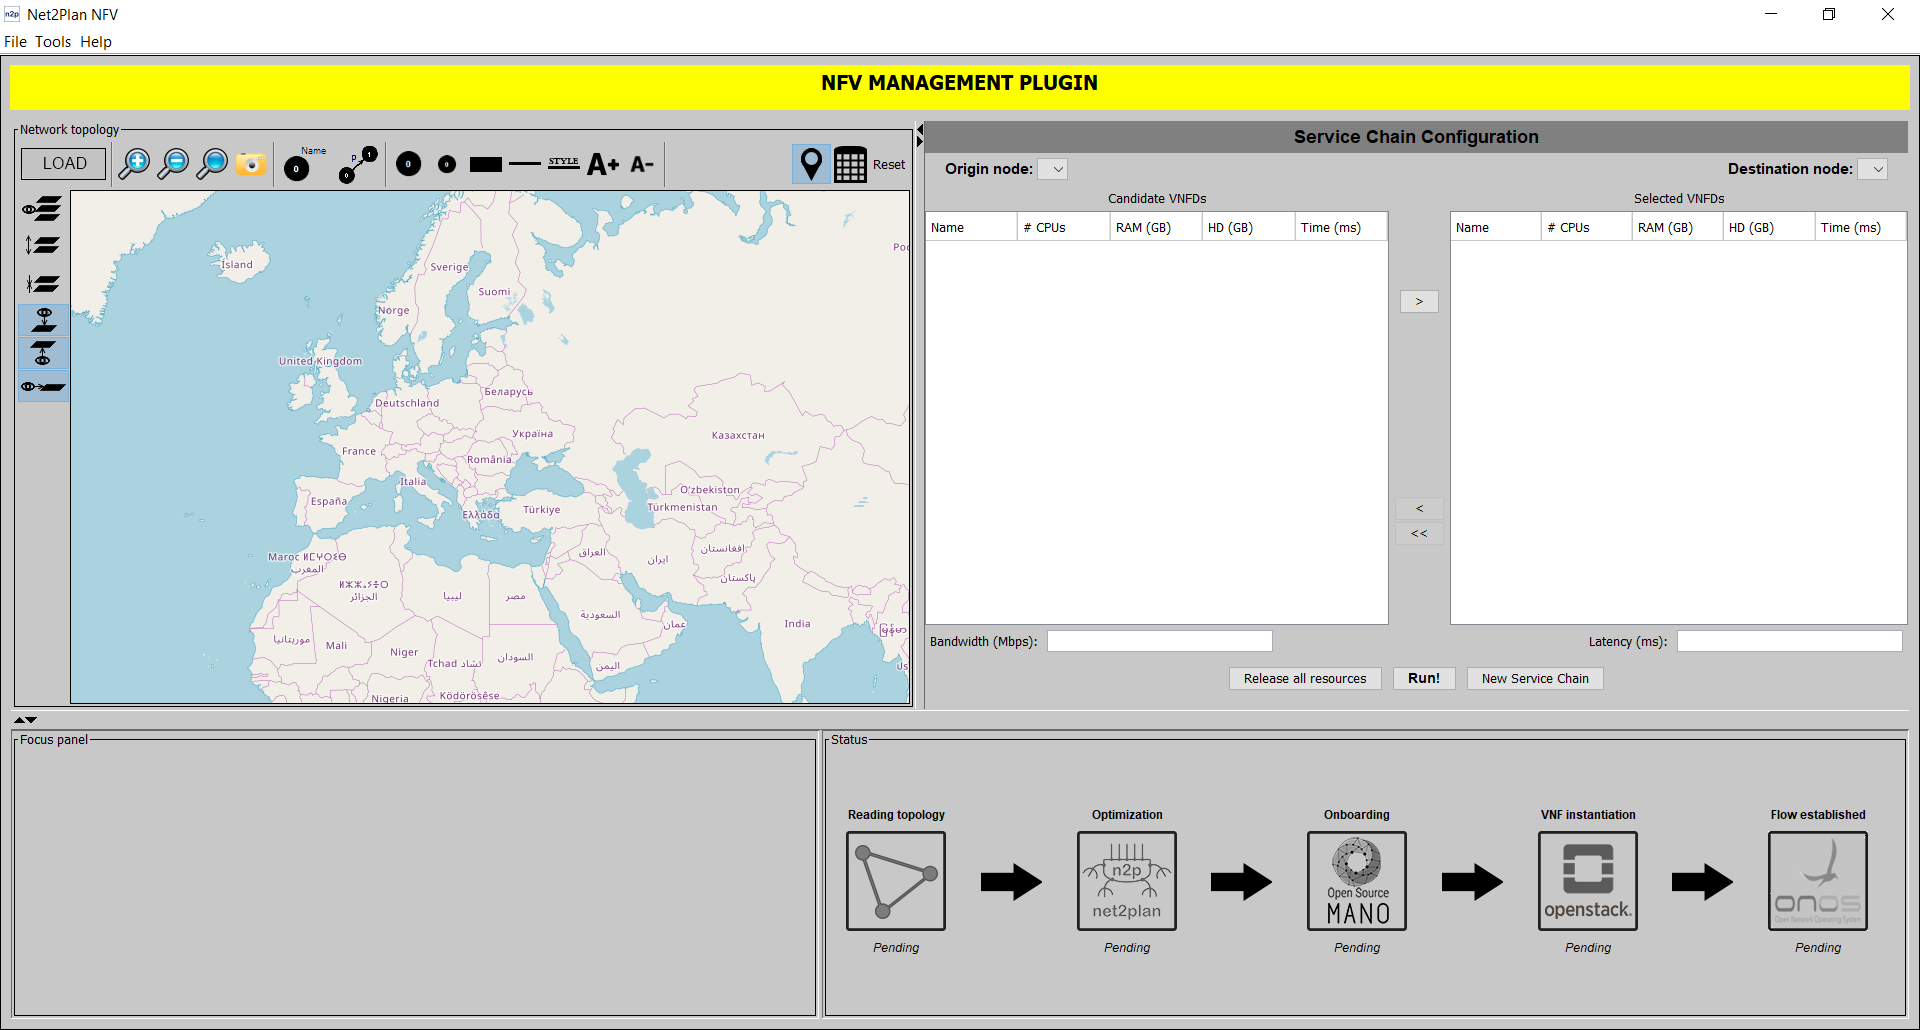
\includegraphics[width=1\linewidth]{imagenes/nfvplugin_dashboard}
	\caption{Interfaz gráfica del Plugin NFV-Management}
	\label{fig:nfvplugindash}
\end{figure}

En la figura \ref{fig:nfvplugindash} se puede observar la interfaz gráfica del Plugin NFV-Management, la cual está dividida en diferentes secciones:

\begin{itemize}
	\item Arriba a la izquierda se encuentra el \textit{TopologyPanel}, que se encarga de dibujar la topología deseada. Esta funcionalidad es heredada del \textit{Plugin Network Design} de Net2Plan.
	
	\item Arriba a la derecha se encuentra el \textit{OSMPanel}, que se encarga de obtener información sobre los distintos NSD que se encuentran disponibles en OSM y mostrarla al usuario de una manera amigable, informándole de que recursos (\ac{HD}, \ac{RAM}, \ac{CPU}) son necesarios para su instanciación en un VIM.
	
	Así mismo, también incluye botones para realizar la ejecución de la prueba de concepto, así como el borrar todos los \acp{VNF} instanciados en \ac{OSM}.
	
	\item Abajo a la izquierda se encuentra el \textit{FocusPanel}, que se encarga de mostrar información detallada de un elemento en concreto cuando se selecciona. Dicha funcionalidad es heredada del \textit{Plugin Network Design} de Net2Plan.
	
	\item Abajo a la derecha se encuentra el \textit{ServiceChainPanel}, que se encarga de mostrar la fase en la que se encuentra el transcurso de la prueba de concepto. 
	
	Hay cinco fases: 
	
	\begin{itemize}
		
		\item La primera indica que se ha cargado la topología de \ac{ONOS} correctamente.
		
		\item La segunda indica que el algoritmo de \ac{NFV} se ha ejecutado correctamente.
		
		\item La tercera indica que los \acp{VNF} se han instanciado correctamente en \ac{OSM}.
		
		\item La cuarta muestra cuando OpenStack ha creado las máquinas virtuales asociadas a los \acp{VNF} instanciados.
		
		\item La quinta fase indica que se han instalado las reglas de flujo en \ac{ONOS} y la \textit{Service Chain} se satisface correctamente.
		
	\end{itemize}

\end{itemize}


\cleardoublepage